\documentclass[11pt,letterpaper]{article}

%\usepackage{subfigure}
\usepackage{graphicx}
\usepackage{amsmath}
\usepackage{amssymb}
\usepackage{enumitem}

%\usepackage{paralist}
%\usepackage{bm}
%\usepackage{cite}
\usepackage{subcaption}
\usepackage{multirow}
\usepackage{umoline}
\usepackage{xspace}
\usepackage{soul}
\usepackage{graphicx}
%\usepackage{url}


\setlength{\textwidth}{6.5in}     
\setlength{\oddsidemargin}{0in}  
\setlength{\evensidemargin}{0in}
\setlength{\textheight}{8.5in} 
\setlength{\topmargin}{0in}   
\setlength{\headheight}{14pt} 
\setlength{\headsep}{10pt}   
%\setlength{\footskip}{0in}

%------------------------------------------------
\newcommand{\homework}[2]{
\setcounter{section}{#1}
\section*{ICS635 Homework {\thesection}: {#2} }
{\markboth{#2}{#2}}
}
%------------------------------------------------


\begin{document}

% Enter the Homework number and title as arguments to
% homework
\homework{4}{by Lambert Leong}

\textbf{Problem 1}
%https://www.quora.com/What-are-the-differences-between-maximum-likelihood-and-cross-entropy-as-a-loss-function
%https://stats.stackexchange.com/questions/364216/the-relationship-between-maximizing-the-likelihood-and-minimizing-the-cross-entro
%http://www.awebb.info/blog/cross_entropy
%https://medium.com/konvergen/cross-entropy-and-maximum-likelihood-estimation-58942b52517a
\\
\\Maximizing the conditional likelihood of the data.
 \begin{align*}
	\mathcal{L}(\mathcal{D})=p_{\theta}(y_{n}|x_{n})& =
\prod_{n}^{N}(\hat{y_{n}})^{y_{n}}(1-\hat{y_{n}})^{1-y_{n}} \\
 	%&= \sum_{n}^{N}(\hat{y_{n}}log(y_{n})+(1-y_{n})log(1-\hat{y_{n}}))
 \end{align*}
Maximizing the log-likelihood
 \begin{align*}
 	log\mathcal{L}(\mathcal{D})= \sum_{n}^{N}(\hat{y_{n}}log(y_{n})+(1-y_{n})log(1-\hat{y_{n}}))
 \end{align*}
Minimizing the binary cross-entropy loss
 \begin{align*}
	L(\mathcal{D})	&= - \frac{1}{N} \sum_{n}^{N}
(\hat{y_{n}}log(y_{n})+(1-y_{n})log(1-\hat{y_{n}})) \\
	- \frac{1}{N}L(\mathcal{D}) &=  \sum_{n}^{N} (\hat{y_{n}}log(y_{n})+(1-y_{n})log(1-\hat{y_{n}}))
 \end{align*}
Therefore, we can say maximizing the log-likelihood is equivalent to minimizing
the binary cross-entropy loss
 \begin{align*}
log\mathcal{L}(\mathcal{D})=- \frac{1}{N}L(\mathcal{D})
 \end{align*}
%\noindent
\textbf{Problem 2}
\begin{enumerate}[labelindent=0pt]
\item
Sample size is large enough to do a 60\%, 20\%, 20\% split for train,
validation, and test.
\item
The exact architecture or neural net model is ambiguous.
\item
The loss function being optimized is not clear.
\item
The exact hyper parameters optimized are not stated.
\item
The evaluation method for the competition is unclear(i.e. are they using AUROC,
AUPRC, or etc).
\item
It seems as though the test set was not used.  The individual does not report
how the tuned model did on the test set. 
\item
It is unclear if the individual is first place on the leader board of if they
actually won the whole competition.
\item
The final optimized parameters are not reported which makes it difficult to
reproduce the work.
\item
It is not clear what data set was used to train the final model that was
submitted.  Did the individual use just the model trained on the 80\% training
data or all the training data? 
\item
The final test set, mentioned in the last line, is ambiguous because it could be
referring to the withheld dataset that is used to pick the winners or the final
test set(10\% of the training) that the individual set aside when he did his data split.
\end{enumerate}

\textbf{Problem 3}
%http://cross-entropy.net/ML310/homework03_answers.txt
\begin{enumerate}[labelindent=0pt]
\item 
Centering data affects the principal components if it is calculated via singular
value decomposition.  However, if one is to compute the principal components by
first computing the covariance matrix then centering should not affect
principal components.

\item 
Scaling data can help prevent one principal component explaining the majority of
the variance.  If the data is not scaled properly, one feature could dominate
and influence the axis of maximal variance. 

\item 
%https://stats.stackexchange.com/questions/359570/equal-covariance-in-linear-discriminant-analysis
Classes will be indistinguishable if the two classes are centered around the
same space with respect to the two dimensions or principal components they are
plotted in.  In other words, if a 2D plot is made using the wrong two
components, it could appear that the 2 Gaussians are superimposed on each other
which would make them appear indistinguishable.  Interchanging one principal
component for a third or plotting in a higher dimension will likely show some
separability.

\begin{figure}[h!]
    \centering
    \begin{subfigure}[]{.3\textwidth}
        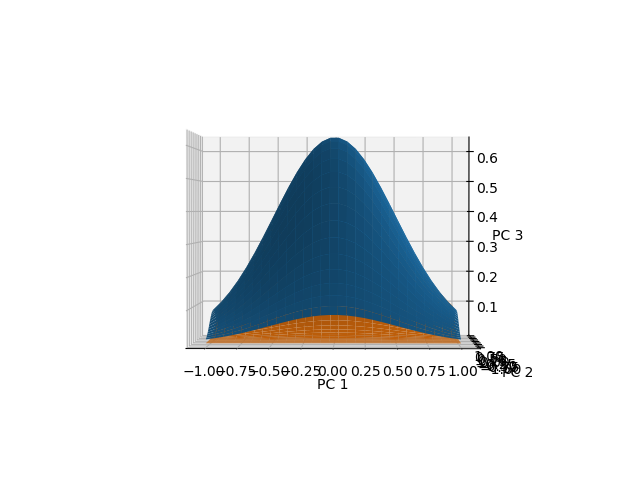
\includegraphics[width=\textwidth]{pc1.png}
        \caption{view of PC1 vs PC3, Indistinguishable}
        \label{fig:}
    \end{subfigure}
   \begin{subfigure}[]{.3\textwidth}
        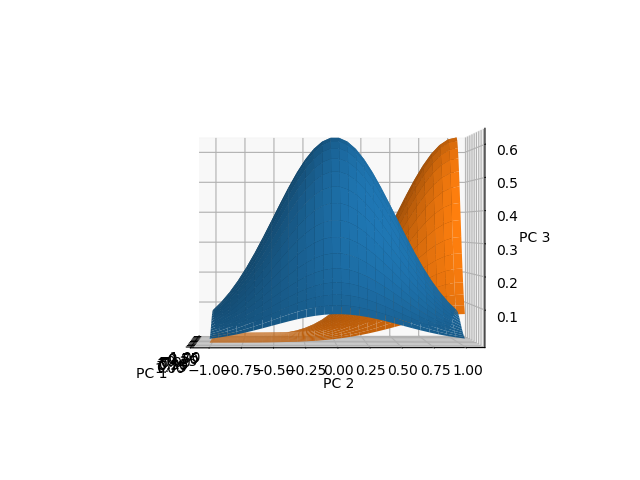
\includegraphics[width=\textwidth]{pc3.png}
        \caption{View of PC2 vs PC3, Class separation visible}
        \label{fig:}
    \end{subfigure}
  \begin{subfigure}[]{.3\textwidth}
        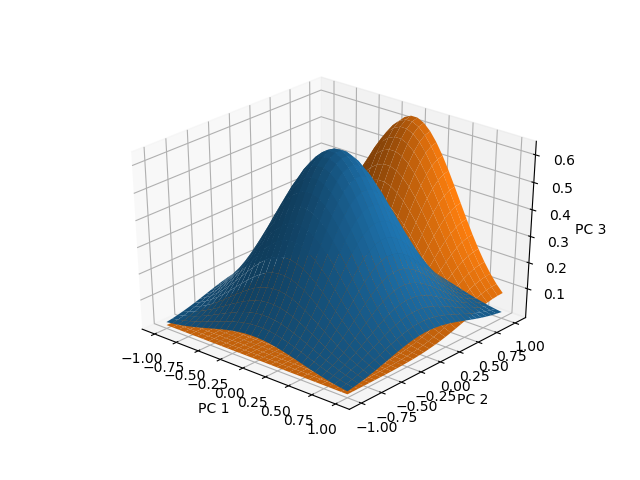
\includegraphics[width=\textwidth]{3d.png}
        \caption{3D plot, Class separation visible}
        \label{fig:}
  \end{subfigure} 
    \caption{Example of how 2D views can lead to indistinguishable classes}
    \label{fig:}
\end{figure}


\item 
If the network is free of any nonlinearities then it is convex.  
It will be equivalent to plotting the data in principal component space.
\end{enumerate}

\textbf{Problem 4}
\begin{enumerate}[labelindent=0pt]
\item 
If you have data points on previous days to construct a reasonable posterior, it
will be better than flipping a coin.
% If you have a proper length parameter - determines similarity between two points, higher means points are more similar.  and sigma, explains variance, higher means bigger confidence area of the function at a given point
\item 
Trusting the oracle can change prediction. If a new Gaussian process is fit with
the addition of new data point, it can narrow the range of your prediction; so
yes it will affect your models prediction.
\item 
MAP
\end{enumerate}


\noindent\end{document}

